\documentclass[tikz,border=6pt]{standalone}
\usepackage{lmodern}
\usepackage[T1]{fontenc}
\usepackage{amssymb}
\usepackage{amsmath}
\usetikzlibrary{arrows.meta,shapes.geometric,fit,backgrounds,calc,positioning,decorations.pathreplacing}
\definecolor{letterA}{HTML}{1F5FA9}
\definecolor{letterB}{HTML}{B5651D}
\definecolor{boxline}{HTML}{B9BEC4}
\definecolor{boxfill}{HTML}{F4F5F7}
\definecolor{kernel}{HTML}{3A3F45}
\definecolor{thetaT}{HTML}{2E7D46}
\definecolor{thetaF}{HTML}{C1443C}
\definecolor{xval}{HTML}{5A6470}
\definecolor{ref}{HTML}{8A9099}
\definecolor{ink}{HTML}{222629}
\tikzset{
  % ---- classes ---------------------------------------------------
  cls/.style        = {circle, draw=ink, line width=.5pt, fill=white,
                       inner sep=0pt, minimum size=13mm, align=center,
                       font=\small},
  bottom/.style     = {cls, double, double distance=1pt},
  kern/.style       = {draw=kernel, line width=1.6pt},
  % ---- SCC boxes -------------------------------------------------
  sccbox/.style     = {rounded corners=3pt, draw=boxline, fill=boxfill,
                       line width=.7pt},
  scctag/.style     = {font=\scriptsize\itshape, text=ref, align=center},
  % ---- alphabet edges --------------------------------------------
  ea/.style         = {draw=letterA, text=letterA, line width=.9pt,
                       -{Stealth[length=2mm]}},
  eb/.style         = {draw=letterB, text=letterB, line width=.9pt,
                       dashed, dash pattern=on 2.4pt off 1.6pt,
                       -{Stealth[length=2mm]}},
  eall/.style       = {draw=ink, text=ink, line width=.9pt,
                       -{Stealth[length=2mm]}},
  elab/.style       = {font=\scriptsize, inner sep=1.5pt,
                       fill=white, fill opacity=.85, text opacity=1},
  % ---- read-off decorations --------------------------------------
  thetaT/.style     = {circle, fill=thetaT, text=white, inner sep=0pt,
                       minimum size=4mm, font=\tiny\bfseries},
  thetaF/.style     = {circle, fill=thetaF, text=white, inner sep=0pt,
                       minimum size=4mm, font=\tiny\bfseries},
  xann/.style       = {font=\footnotesize, text=xval},
  result/.style     = {font=\small, text=ink},
  % ---- word ruler / verdict panels (FIG-2, FIG-3) ----------------
  cut/.style        = {draw=ref, line width=.8pt},
  jcut/.style       = {draw=ink, line width=1.1pt},
  cell/.style       = {font=\small\ttfamily, text=ink, inner sep=1pt},
  hi/.style         = {rounded corners=1pt, fill=letterA, fill opacity=.14},
  brk/.style        = {draw=ref, line width=.7pt,
                       decorate, decoration={brace, amplitude=4pt}},
  vrow/.style       = {font=\small, text=ink, anchor=west},
  vnote/.style      = {font=\scriptsize\itshape, text=ref, anchor=west},
}

\begin{document}
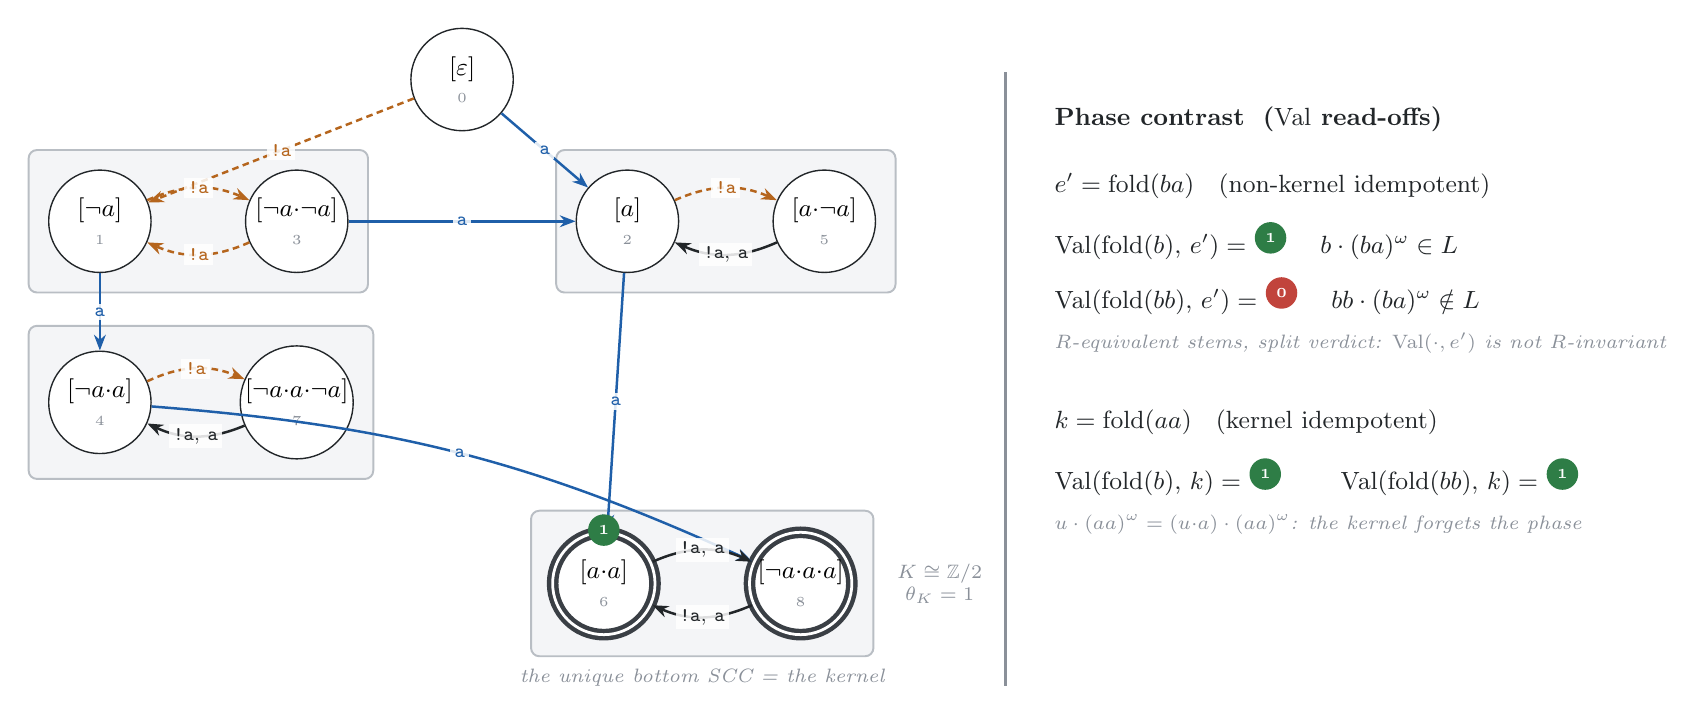
\begin{tikzpicture}
\begin{scope}[scale=1.0]
  \node[cls] (c0) at (0.00,4.40) {$[\varepsilon]$\\[-1pt]\textcolor{ref}{\tiny 0}};
  \node[cls] (c1) at (-4.60,2.60) {$[\lnot a]$\\[-1pt]\textcolor{ref}{\tiny 1}};
  \node[cls] (c2) at (2.10,2.60) {$[a]$\\[-1pt]\textcolor{ref}{\tiny 2}};
  \node[cls] (c3) at (-2.10,2.60) {$[\lnot a{\cdot}\lnot a]$\\[-1pt]\textcolor{ref}{\tiny 3}};
  \node[cls] (c4) at (-4.60,0.30) {$[\lnot a{\cdot}a]$\\[-1pt]\textcolor{ref}{\tiny 4}};
  \node[cls] (c5) at (4.60,2.60) {$[a{\cdot}\lnot a]$\\[-1pt]\textcolor{ref}{\tiny 5}};
  \node[bottom,kern] (c6) at (1.80,-2.00) {$[a{\cdot}a]$\\[-1pt]\textcolor{ref}{\tiny 6}};
  \node[cls] (c7) at (-2.10,0.30) {$[\lnot a{\cdot}a{\cdot}\lnot a]$\\[-1pt]\textcolor{ref}{\tiny 7}};
  \node[bottom,kern] (c8) at (4.30,-2.00) {$[\lnot a{\cdot}a{\cdot}a]$\\[-1pt]\textcolor{ref}{\tiny 8}};
  \draw[eb] (c0) to node[elab] {\texttt{!a}} (c1);
  \draw[ea] (c0) to node[elab] {\texttt{a}} (c2);
  \draw[eb] (c1) to[bend left=24] node[elab] {\texttt{!a}} (c3);
  \draw[ea] (c1) to node[elab] {\texttt{a}} (c4);
  \draw[eb] (c2) to[bend left=24] node[elab] {\texttt{!a}} (c5);
  \draw[ea] (c2) to node[elab] {\texttt{a}} (c6);
  \draw[eb] (c3) to[bend left=24] node[elab] {\texttt{!a}} (c1);
  \draw[ea] (c3) to node[elab] {\texttt{a}} (c2);
  \draw[eb] (c4) to[bend left=24] node[elab] {\texttt{!a}} (c7);
  \draw[ea] (c4) to[bend left=10] node[elab] {\texttt{a}} (c8);
  \draw[eall] (c5) to[bend left=24] node[elab] {\texttt{!a}, \texttt{a}} (c2);
  \draw[eall] (c6) to[bend left=24] node[elab] {\texttt{!a}, \texttt{a}} (c8);
  \draw[eall] (c7) to[bend left=24] node[elab] {\texttt{!a}, \texttt{a}} (c4);
  \draw[eall] (c8) to[bend left=24] node[elab] {\texttt{!a}, \texttt{a}} (c6);
  \begin{scope}[on background layer]
    \node[sccbox, fit=(c6) (c8), inner sep=7pt] (S6) {};
  \end{scope}
  \begin{scope}[on background layer]
    \node[sccbox, fit=(c2) (c5), inner sep=7pt] (S2) {};
  \end{scope}
  \begin{scope}[on background layer]
    \node[sccbox, fit=(c4) (c7), inner sep=7pt] (S4) {};
  \end{scope}
  \begin{scope}[on background layer]
    \node[sccbox, fit=(c1) (c3), inner sep=7pt] (S1) {};
  \end{scope}
  \node[thetaT] at (c6.north) {1};
\end{scope}
  \node[scctag, anchor=west] at (5.4,-2.0) {$K \cong \mathbb{Z}/2$\\$\theta_K = 1$};
  \node[scctag] at (3.05,-3.2) {the unique bottom SCC = the kernel};
  \node[vrow,font=\small\bfseries] at (7.4,3.9) {Phase contrast \;($\mathrm{Val}$ read-offs)};
  \node[vrow] at (7.4,3.05) {$e' = \mathrm{fold}(ba)$ \; (non-kernel idempotent)};
  \node[vrow] at (7.4,2.3499999999999996) {$\mathrm{Val}(\mathrm{fold}(b),\,e') = $ \tikz\node[thetaT]{1}; \quad $b\cdot(ba)^\omega \in L$};
  \node[vrow] at (7.4,1.6499999999999997) {$\mathrm{Val}(\mathrm{fold}(bb),\,e') = $ \tikz\node[thetaF]{0}; \quad $bb\cdot(ba)^\omega \notin L$};
  \node[vnote] at (7.4,1.0499999999999998) {$R$-equivalent stems, split verdict: $\mathrm{Val}(\cdot,e')$ is not $R$-invariant};
  \node[vrow] at (7.4,0.04999999999999982) {$k = \mathrm{fold}(aa)$ \; (kernel idempotent)};
  \node[vrow] at (7.4,-0.6500000000000001) {$\mathrm{Val}(\mathrm{fold}(b),\,k) = $ \tikz\node[thetaT]{1}; \qquad $\mathrm{Val}(\mathrm{fold}(bb),\,k) = $ \tikz\node[thetaT]{1};};
  \node[vnote] at (7.4,-1.25) {$u\cdot(aa)^\omega = (u{\cdot}a)\cdot(aa)^\omega$: the kernel forgets the phase};
  \draw[cut] (6.9,-3.3) -- (6.9,4.5);
\end{tikzpicture}
\end{document}
